\documentclass[UTF8]{ctexart}
\usepackage{amsmath}
\usepackage{graphicx}
\usepackage{exercise}
\usepackage{hyperref}

\title{贝叶斯统计基础}
\author{沈明宏 (mhshenaa@connect.ust.hk)\\香港科技大学(广州)}
\date{\today}

\begin{document}

\maketitle
\tableofcontents

\vspace{6cm}
\begin{center}
	本文在很大程度上基于澳门大学徐峻教授的贝叶斯课程。
\end{center}

\newpage
\section{概率论基础}

假设一共投了 $S$ 次硬币,其中硬币朝上的次数为 $H$,则硬币朝上的概率 $P(H)$ 为

\begin{equation}
	\begin{aligned}
		P(H) & = \frac{H}{S}
	\end{aligned}
\end{equation}

显然有:

\begin{equation}
	0 \leq P(H) \leq 1
\end{equation}

\begin{center}
	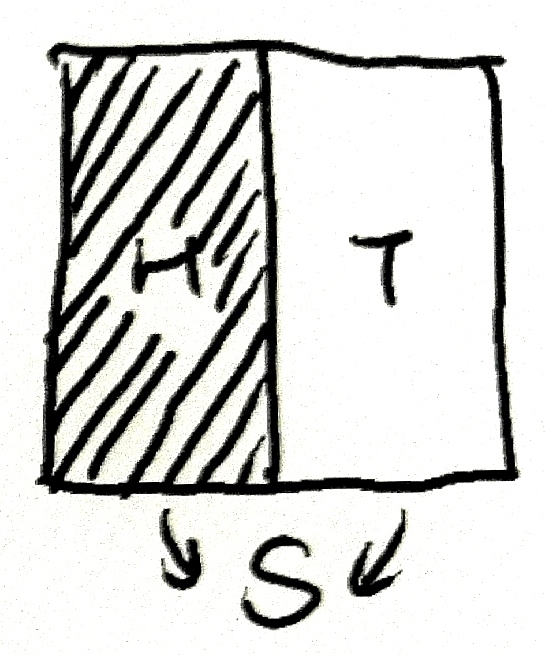
\includegraphics[width=0.25\textwidth]{fig1.jpg}
\end{center}

假设我们让两个人分别投硬币,第一个人投硬币的次数为 $S_1$,第二个人投硬币的次数为 $S_2$,则两个人投硬币朝上的次数分别为 $H_1$ 和 $H_2$,则两个人投硬币朝上的概率 $P(H_1)$ 和 $P(H_2)$ 分别为:

\begin{equation}
	\begin{aligned}
		P(H_1) & = \frac{H_1}{S_1} \\
		P(H_2) & = \frac{H_2}{S_2}
	\end{aligned}
\end{equation}

\begin{center}
	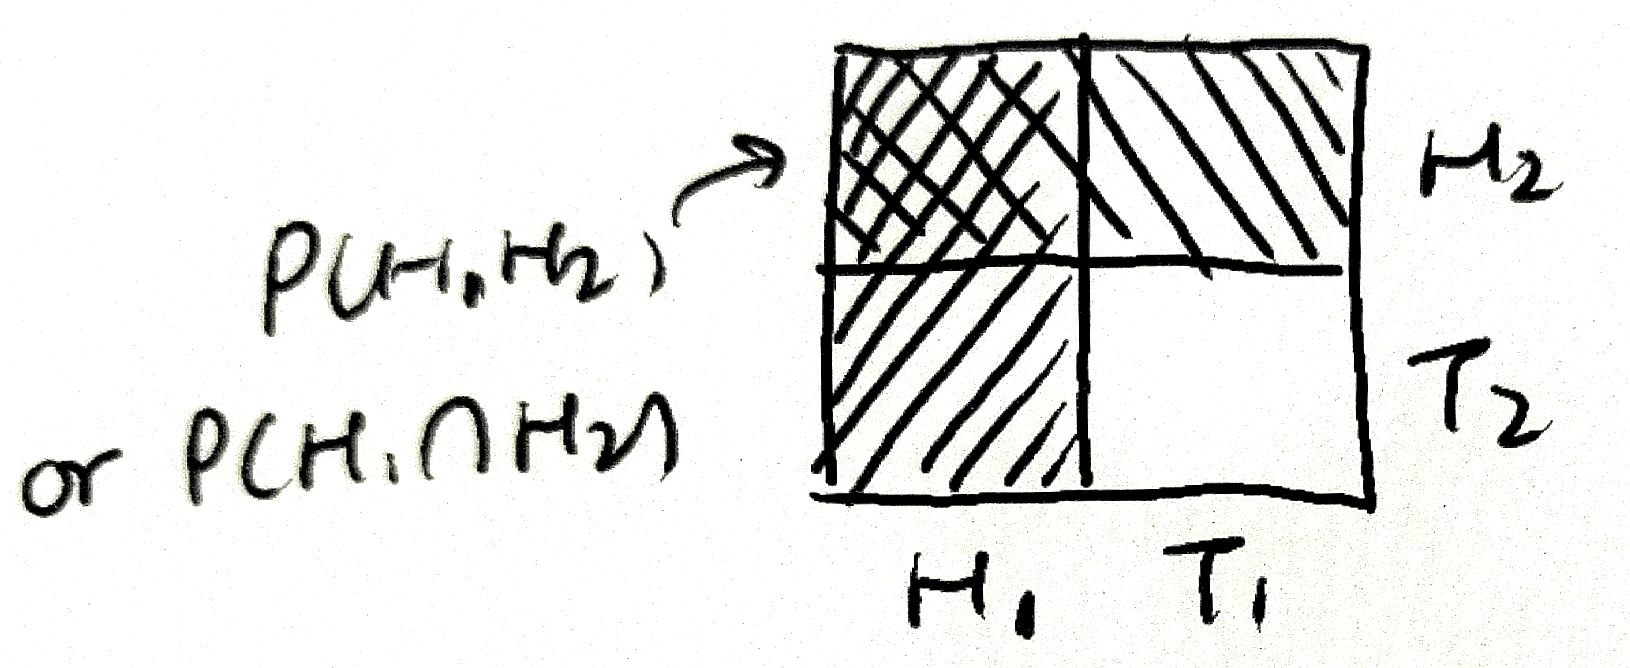
\includegraphics[width=0.6\textwidth]{fig2.jpg}
\end{center}

我们可以计算两个人各投一枚硬币,都朝上的概率 $P(H_1 H_2)$ 为:

\begin{equation}
	\begin{aligned}
		P(H_1 H_2) & = P(H_1 \cap H_2)         \\
		           & = \frac{H_1 H_2}{S_1 S_2}
	\end{aligned}
\end{equation}

同理,我们可以计算下雨的概率 $P(\text{雨})$、带伞的概率 $P(\text{伞})$ 等。

\begin{equation}
	\begin{aligned}
		P(\text{雨}) & = \frac{\text{下雨天数}}{\text{总天数}} \\
		P(\text{伞}) & = \frac{\text{带伞人数}}{\text{总人数}}
	\end{aligned}
\end{equation}

显然,有:

\begin{equation}
	\begin{aligned}
		P(\text{雨}) + P(\text{不下雨}) & = 1 \\
		P(\text{伞}) + P(\text{不带伞}) & = 1
	\end{aligned}
\end{equation}

注意,这里和上面 $P(H)$ 不同,这里的 $P(\text{雨})$ 和 $P(\text{伞})$ 是相关的。

\begin{center}
	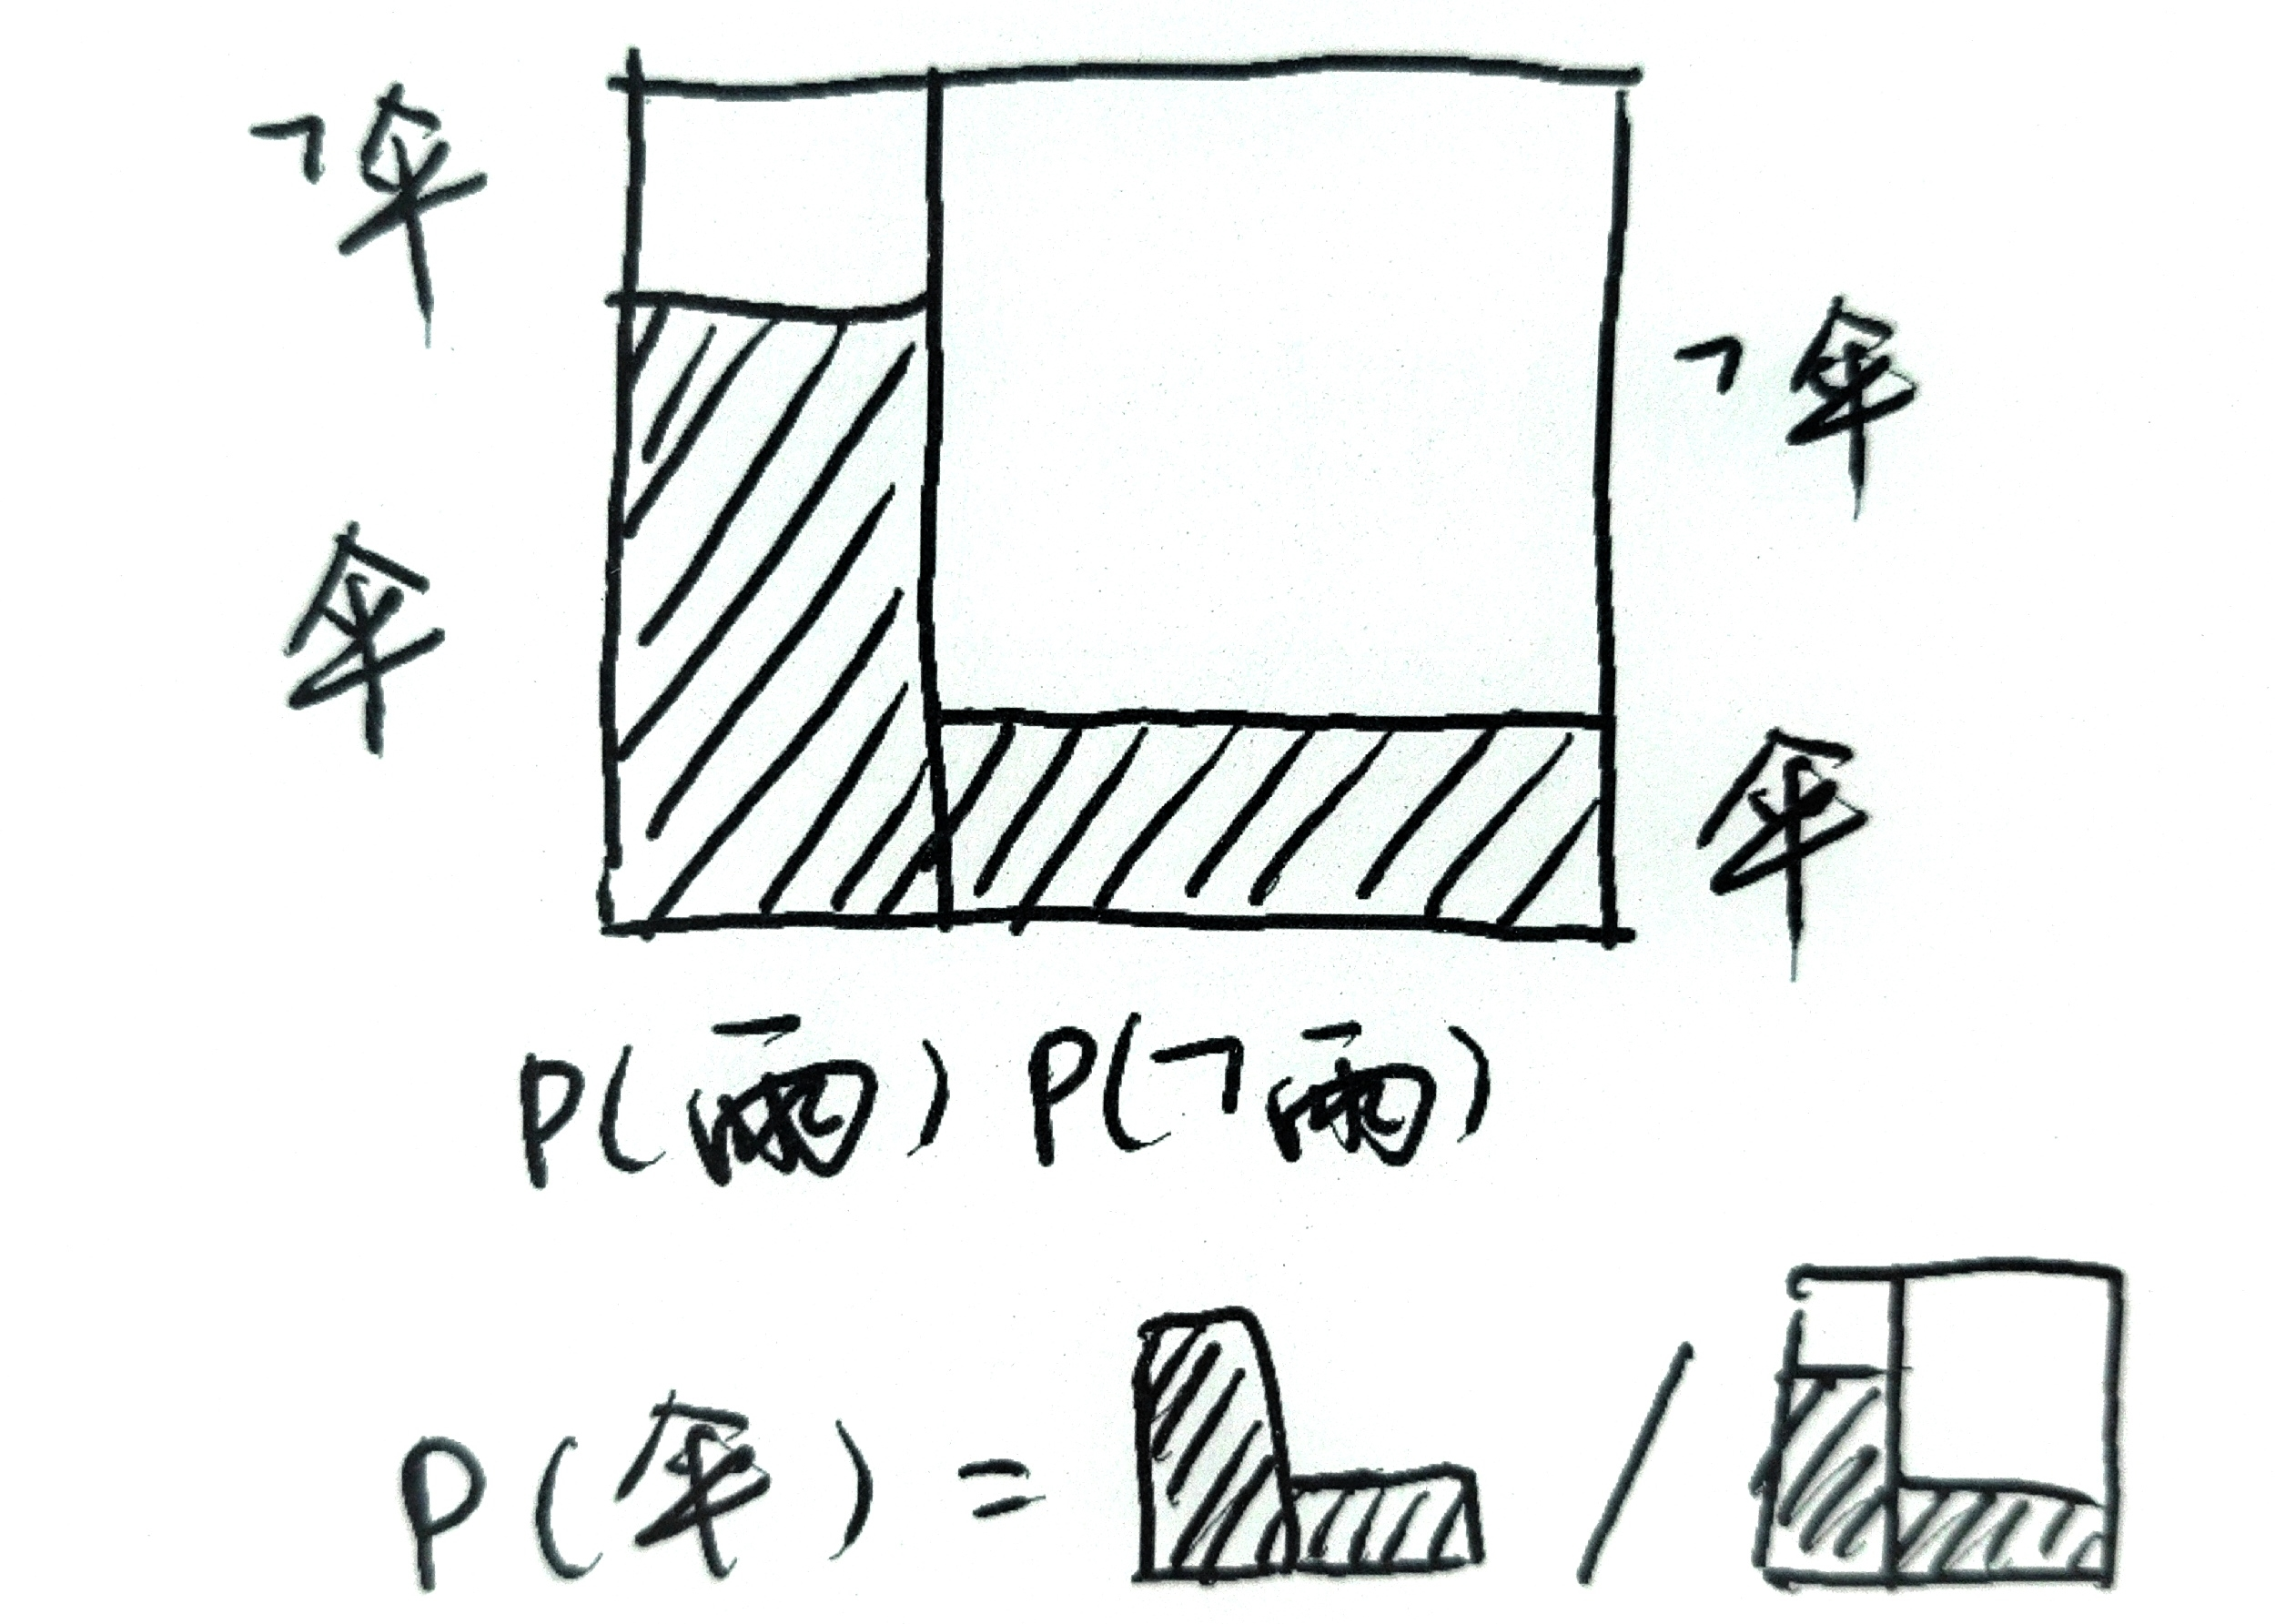
\includegraphics[width=0.5\textwidth]{fig4.jpg}
\end{center}

这时,为了计算两根阴影柱子的高度,我们需要引入“条件概率”。比方说,我们想知道下雨的情况下带伞的概率 $P(\text{伞}|\text{雨})$,则有:

\begin{equation}
	\begin{aligned}
		P(\text{伞}|\text{雨}) & = \frac{P(\text{雨} \cap \text{伞})}{P(\text{雨})} \\
		P(\text{雨}|\text{伞}) & = \frac{P(\text{雨} \cap \text{伞})}{P(\text{伞})}
	\end{aligned}
\end{equation}

\begin{center}
	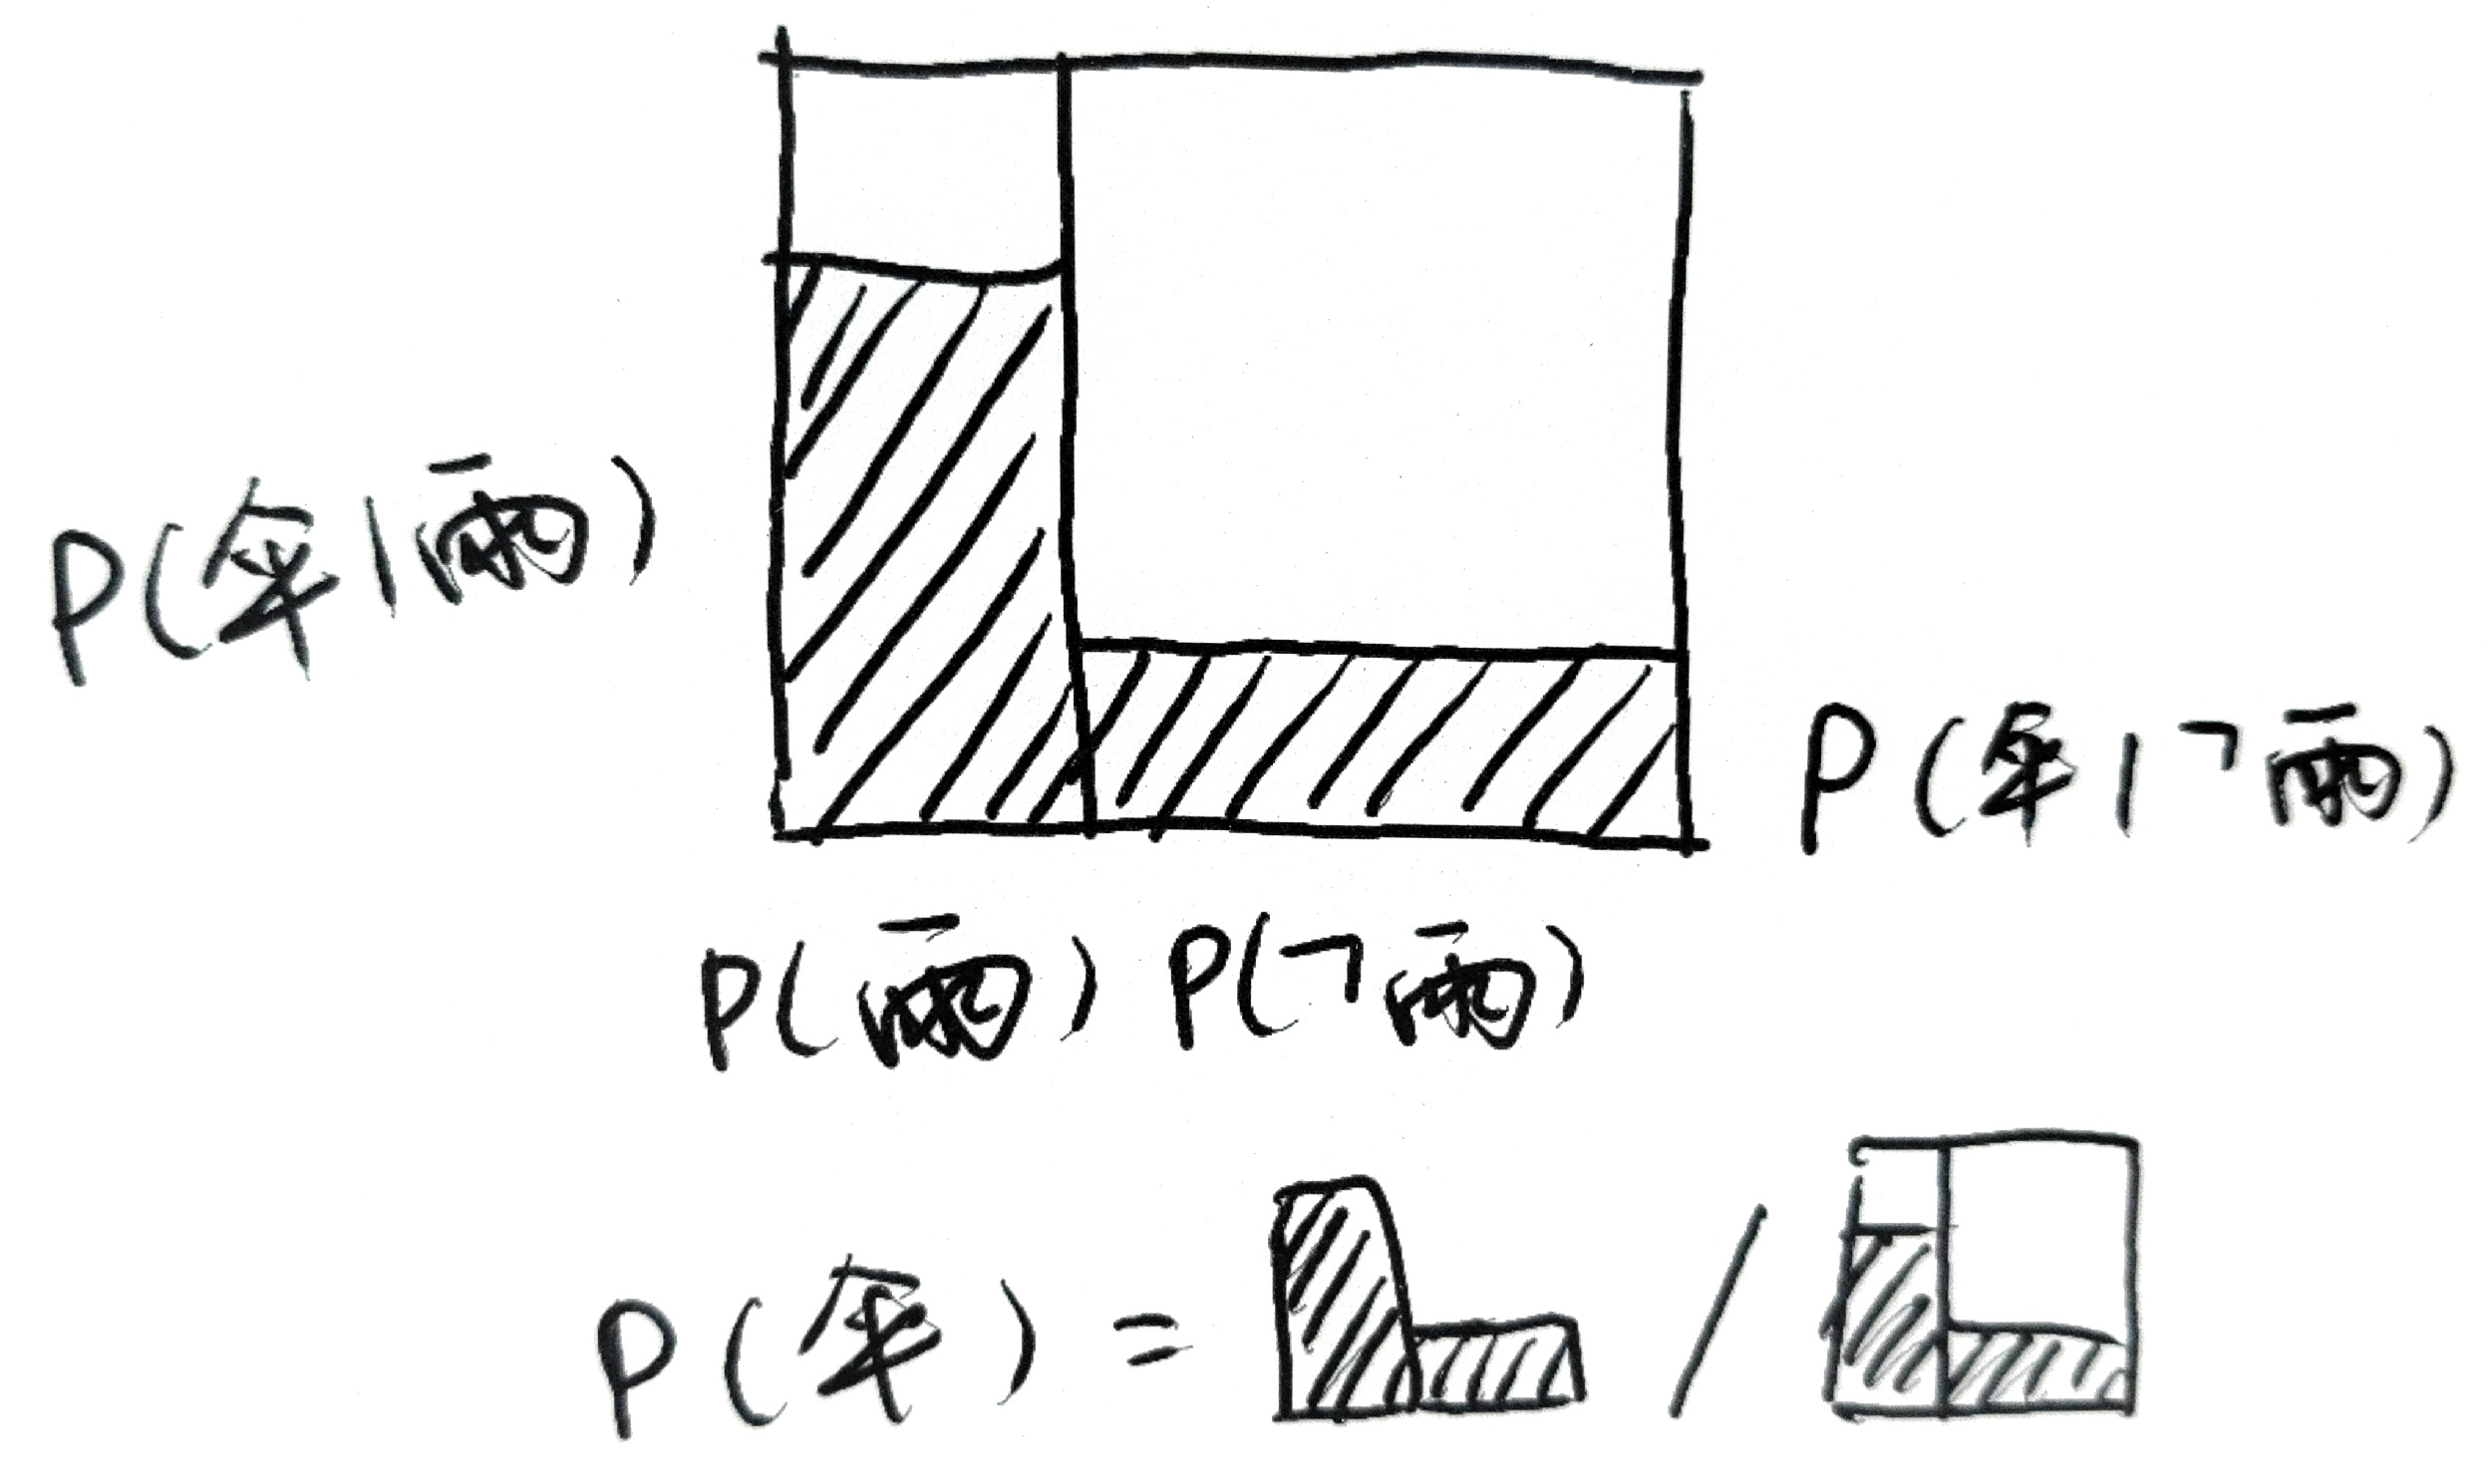
\includegraphics[width=0.6\textwidth]{fig5.jpg}
\end{center}

\newpage
\section{概率分布}

刚才的事件都是离散的,但是在实际中,我们通常会遇到连续的情况。这时,我们就需要引入概率密度函数(PDF)和概率分布函数(CDF)。

\begin{center}
	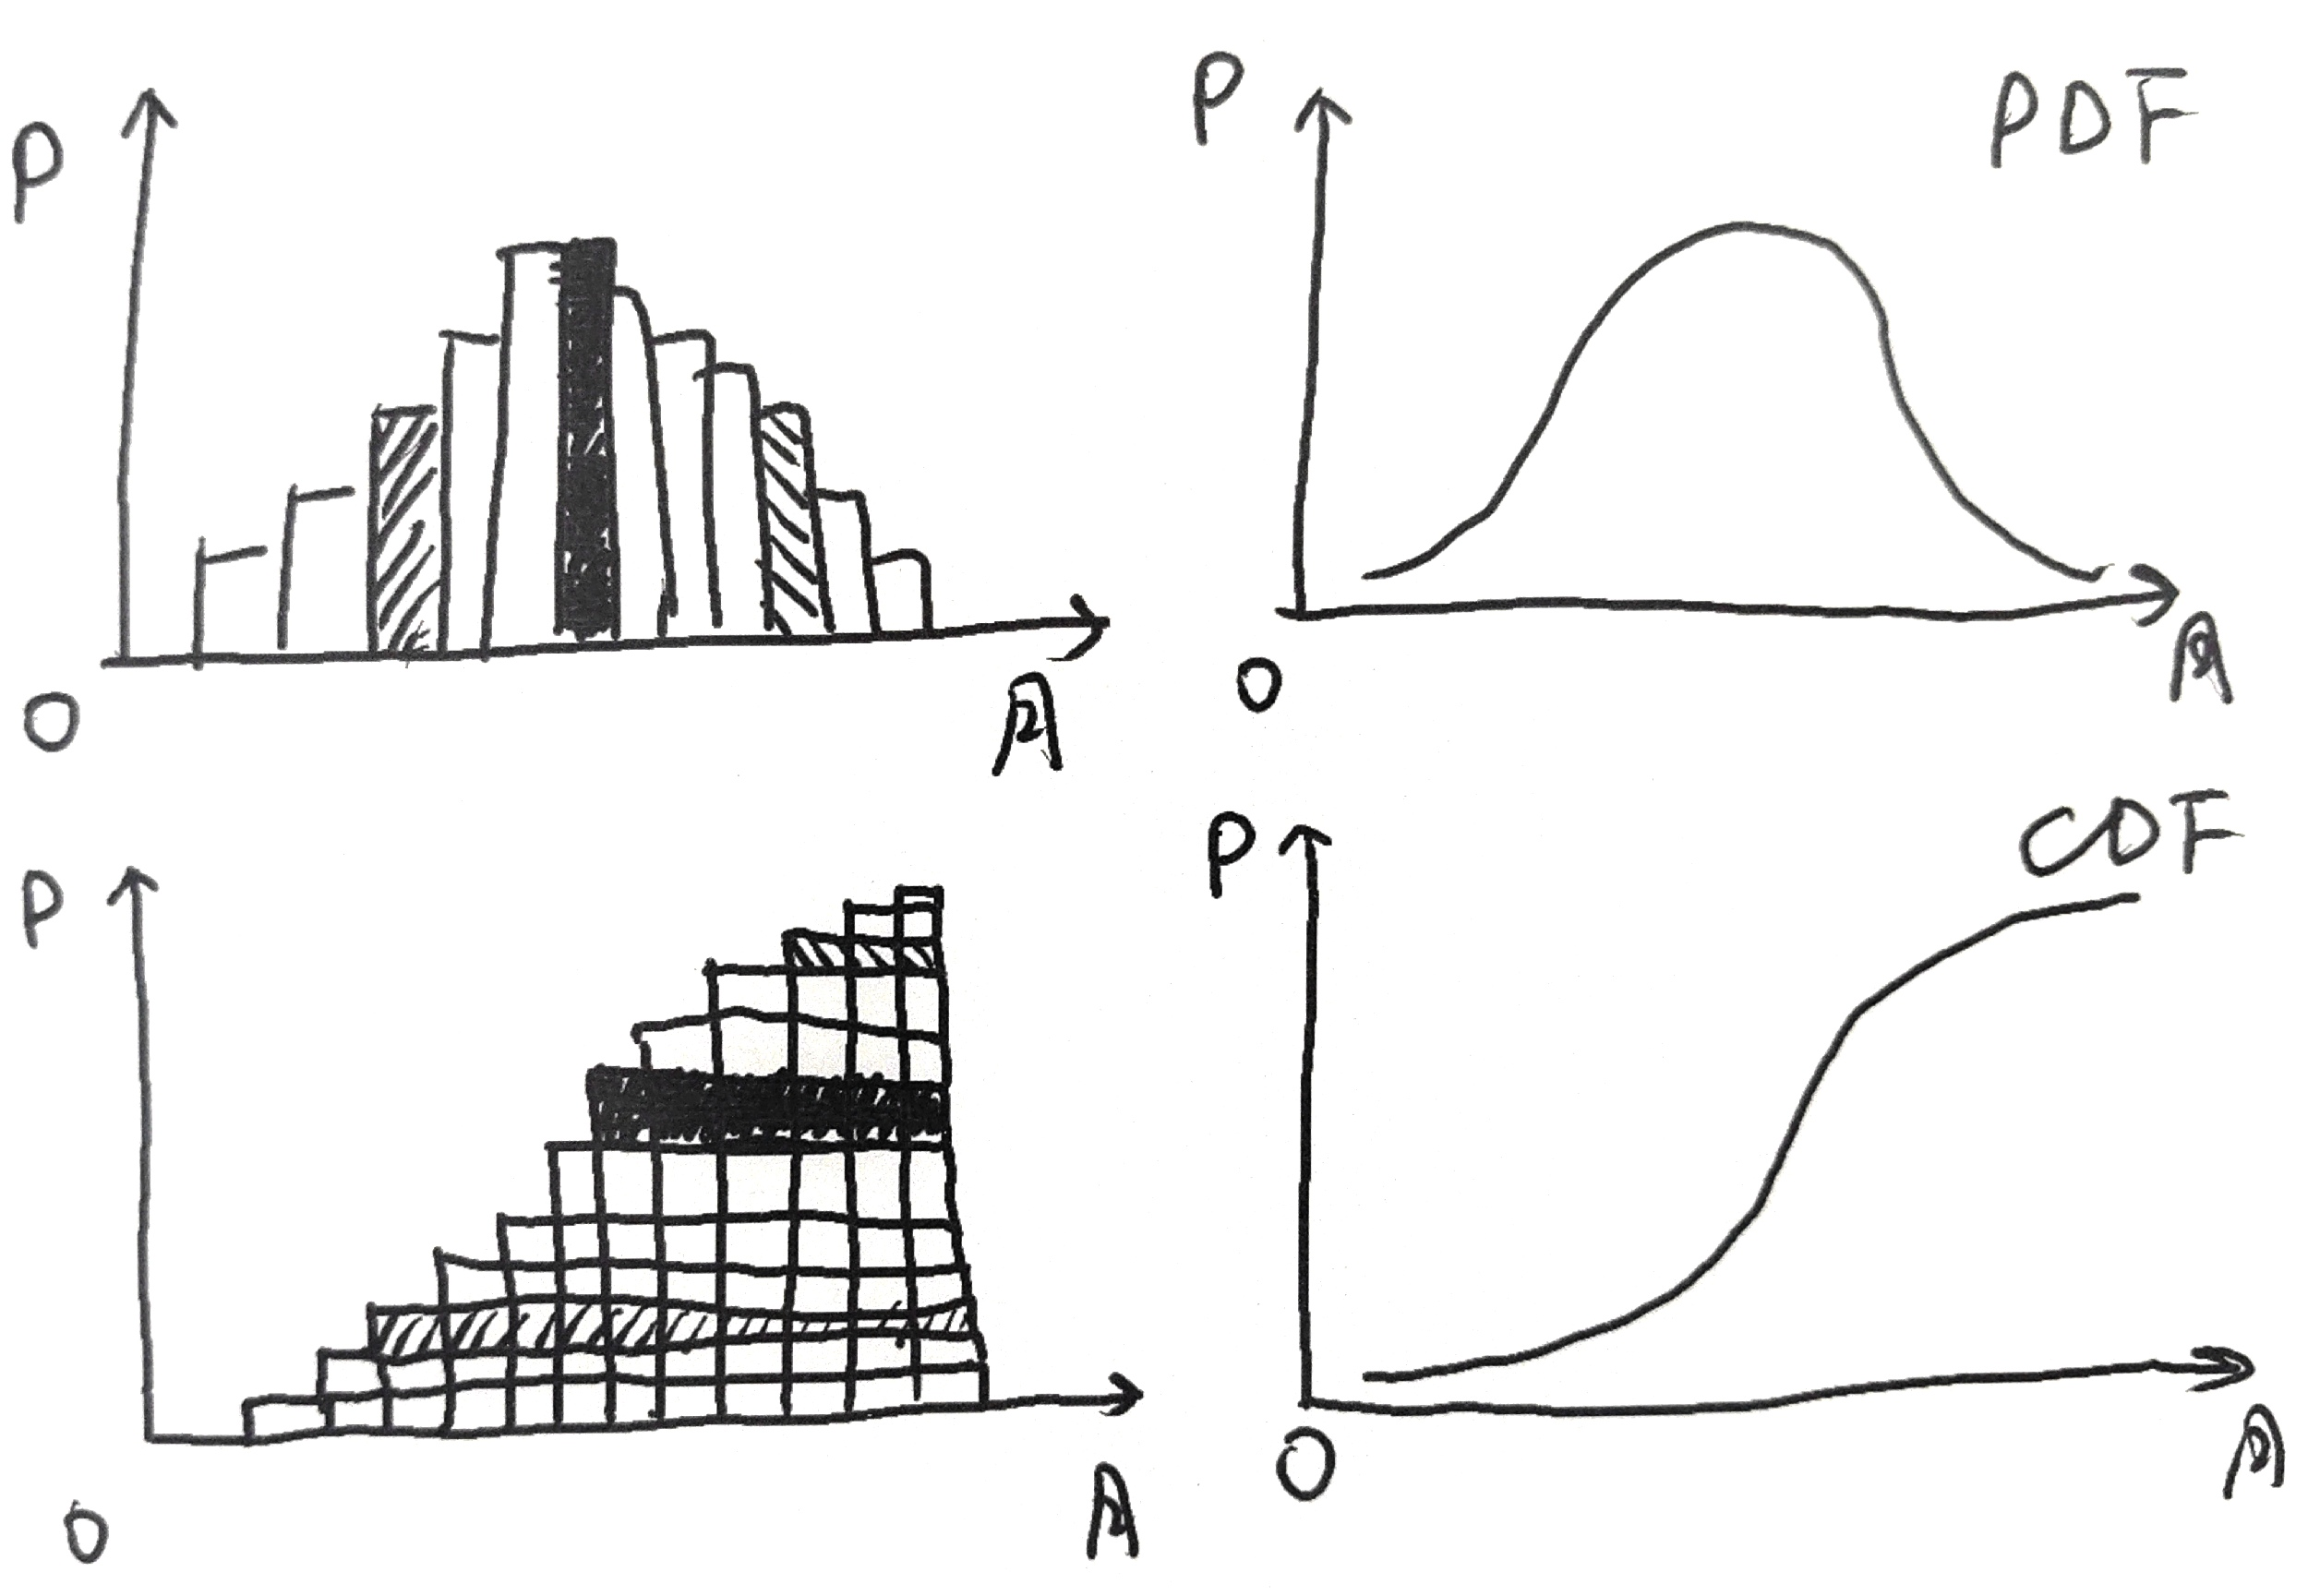
\includegraphics[width=0.75\textwidth]{fig2a.jpg}
\end{center}

概率密度函数 $f(x)$ 是一个函数,满足:

\begin{equation}
	\begin{aligned}
		f(x)                                & \geq 0 \\
		\int_{-\infty}^{+\infty} f(x) \, dx & = 1
	\end{aligned}
\end{equation}

概率分布函数 $F(x)$ 是一个函数,满足:

\begin{equation}
	\begin{aligned}
		F(x) & = \int_{-\infty}^{x} f(x) \, dx
	\end{aligned}
\end{equation}

概率分布函数是概率密度函数的积分,所以有:

\begin{equation}
	\begin{aligned}
		F(b) - F(a) = P(a \leq x \leq b) & = \int_{a}^{b} f(x) \, dx
	\end{aligned}
\end{equation}

反之,如果我们知道概率分布函数 $F(x)$,则可以通过求导得到概率密度函数 $f(x)$:

\begin{equation}
	\begin{aligned}
		f(x) & = \frac{dF(x)}{dx}
	\end{aligned}
\end{equation}


\newpage
\section{贝叶斯定理}

$P(\text{雨}|\text{伞})$ 是个非常奇怪的概率,什么叫“带伞的时候下雨的概率”?

但其实,这才是我们科研中在做的。我们通常是只能收集到“带伞”的数据,然后根据这个数据来推断下雨的概率。

这时,我们就需要用到贝叶斯定理。

根据上面的方程,我们可以得到:

\begin{equation}
	\begin{aligned}
		P(\text{雨} \cap \text{伞})
		 & = P(\text{雨}|\text{伞}) \times P(\text{伞}) \\
		 & = P(\text{伞}|\text{雨}) \times P(\text{雨})
	\end{aligned}
\end{equation}

\begin{center}
	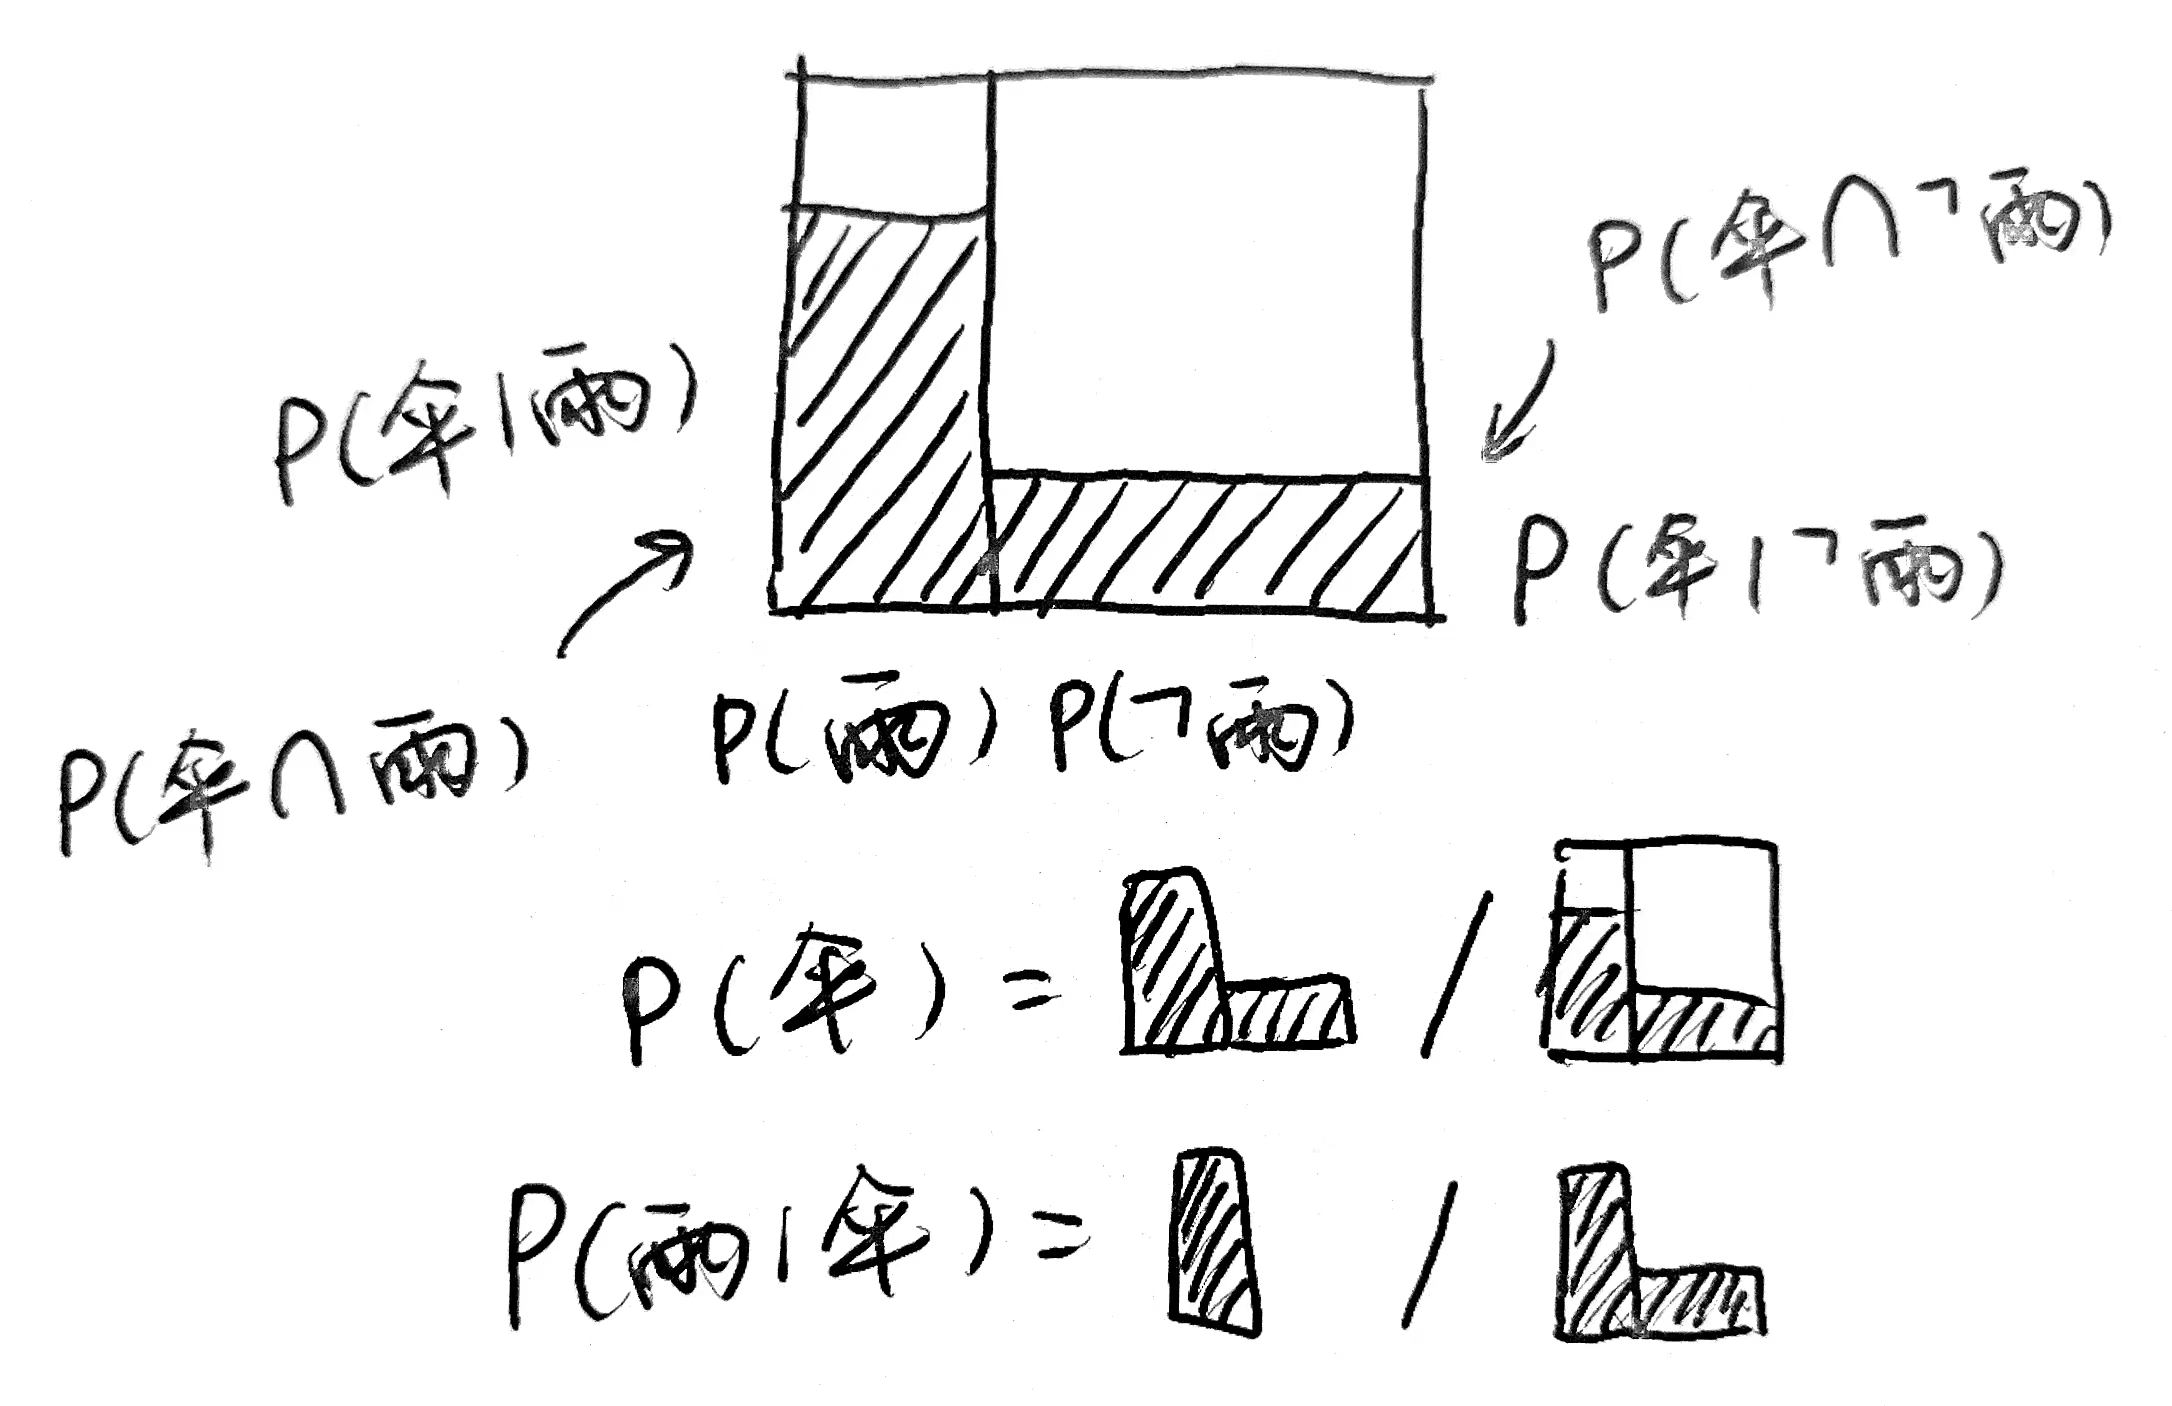
\includegraphics[width=0.8\textwidth]{fig6.jpg}
\end{center}

也就是说:

\begin{equation}
	\begin{aligned}
		P(\text{雨}|\text{伞}) \times P(\text{伞}) & = P(\text{伞}|\text{雨}) \times P(\text{雨})                     \\
		P(\text{雨}|\text{伞})                    & = \frac{P(\text{伞}|\text{雨}) \times P(\text{雨})}{P(\text{伞})}
	\end{aligned}
\end{equation}

这可以抽象为:

\begin{equation}
	\begin{aligned}
		P(\text{参数}|\text{数据}) & = \frac{P(\text{数据}|\text{参数}) \times P(\text{参数})}{P(\text{数据})}
	\end{aligned}
\end{equation}

这是因为 $P(\text{数据})$ 是一个常数,所以在算概率分布的时候可以不用管。

\begin{equation}
	\begin{aligned}
		P(\text{参数}|\text{数据}) & \propto P(\text{数据}|\text{参数}) \times P(\text{参数})
	\end{aligned}
\end{equation}

如果用 $D$ 表示数据,$\theta$ 表示参数,则有:

\begin{equation}
	\begin{aligned}
		P(\theta|D) & \propto P(D|\theta) \times P(\theta)
	\end{aligned}
\end{equation}

这就是贝叶斯定理的核心。

\begin{itemize}
	\item 先验概率(Prior):我们对参数的初始估计 $P(\theta)$
	\item 似然函数(Likelihood):数据在参数下的概率 $P(D|\theta)$
	\item 后验概率(Posterior):我们对参数的最终估计 $P(\theta|D)$
\end{itemize}

\subsection{案例一:核酸检测}

\begin{Exercise}
	小贝去做核酸检测。已知新冠的确诊率为 0.0001,确诊人群的阳性率为 0.99,其他人的阳性率为 0.01。假设小贝的检测结果为阳性,求小贝确诊的概率。
\end{Exercise}

\begin{center}
	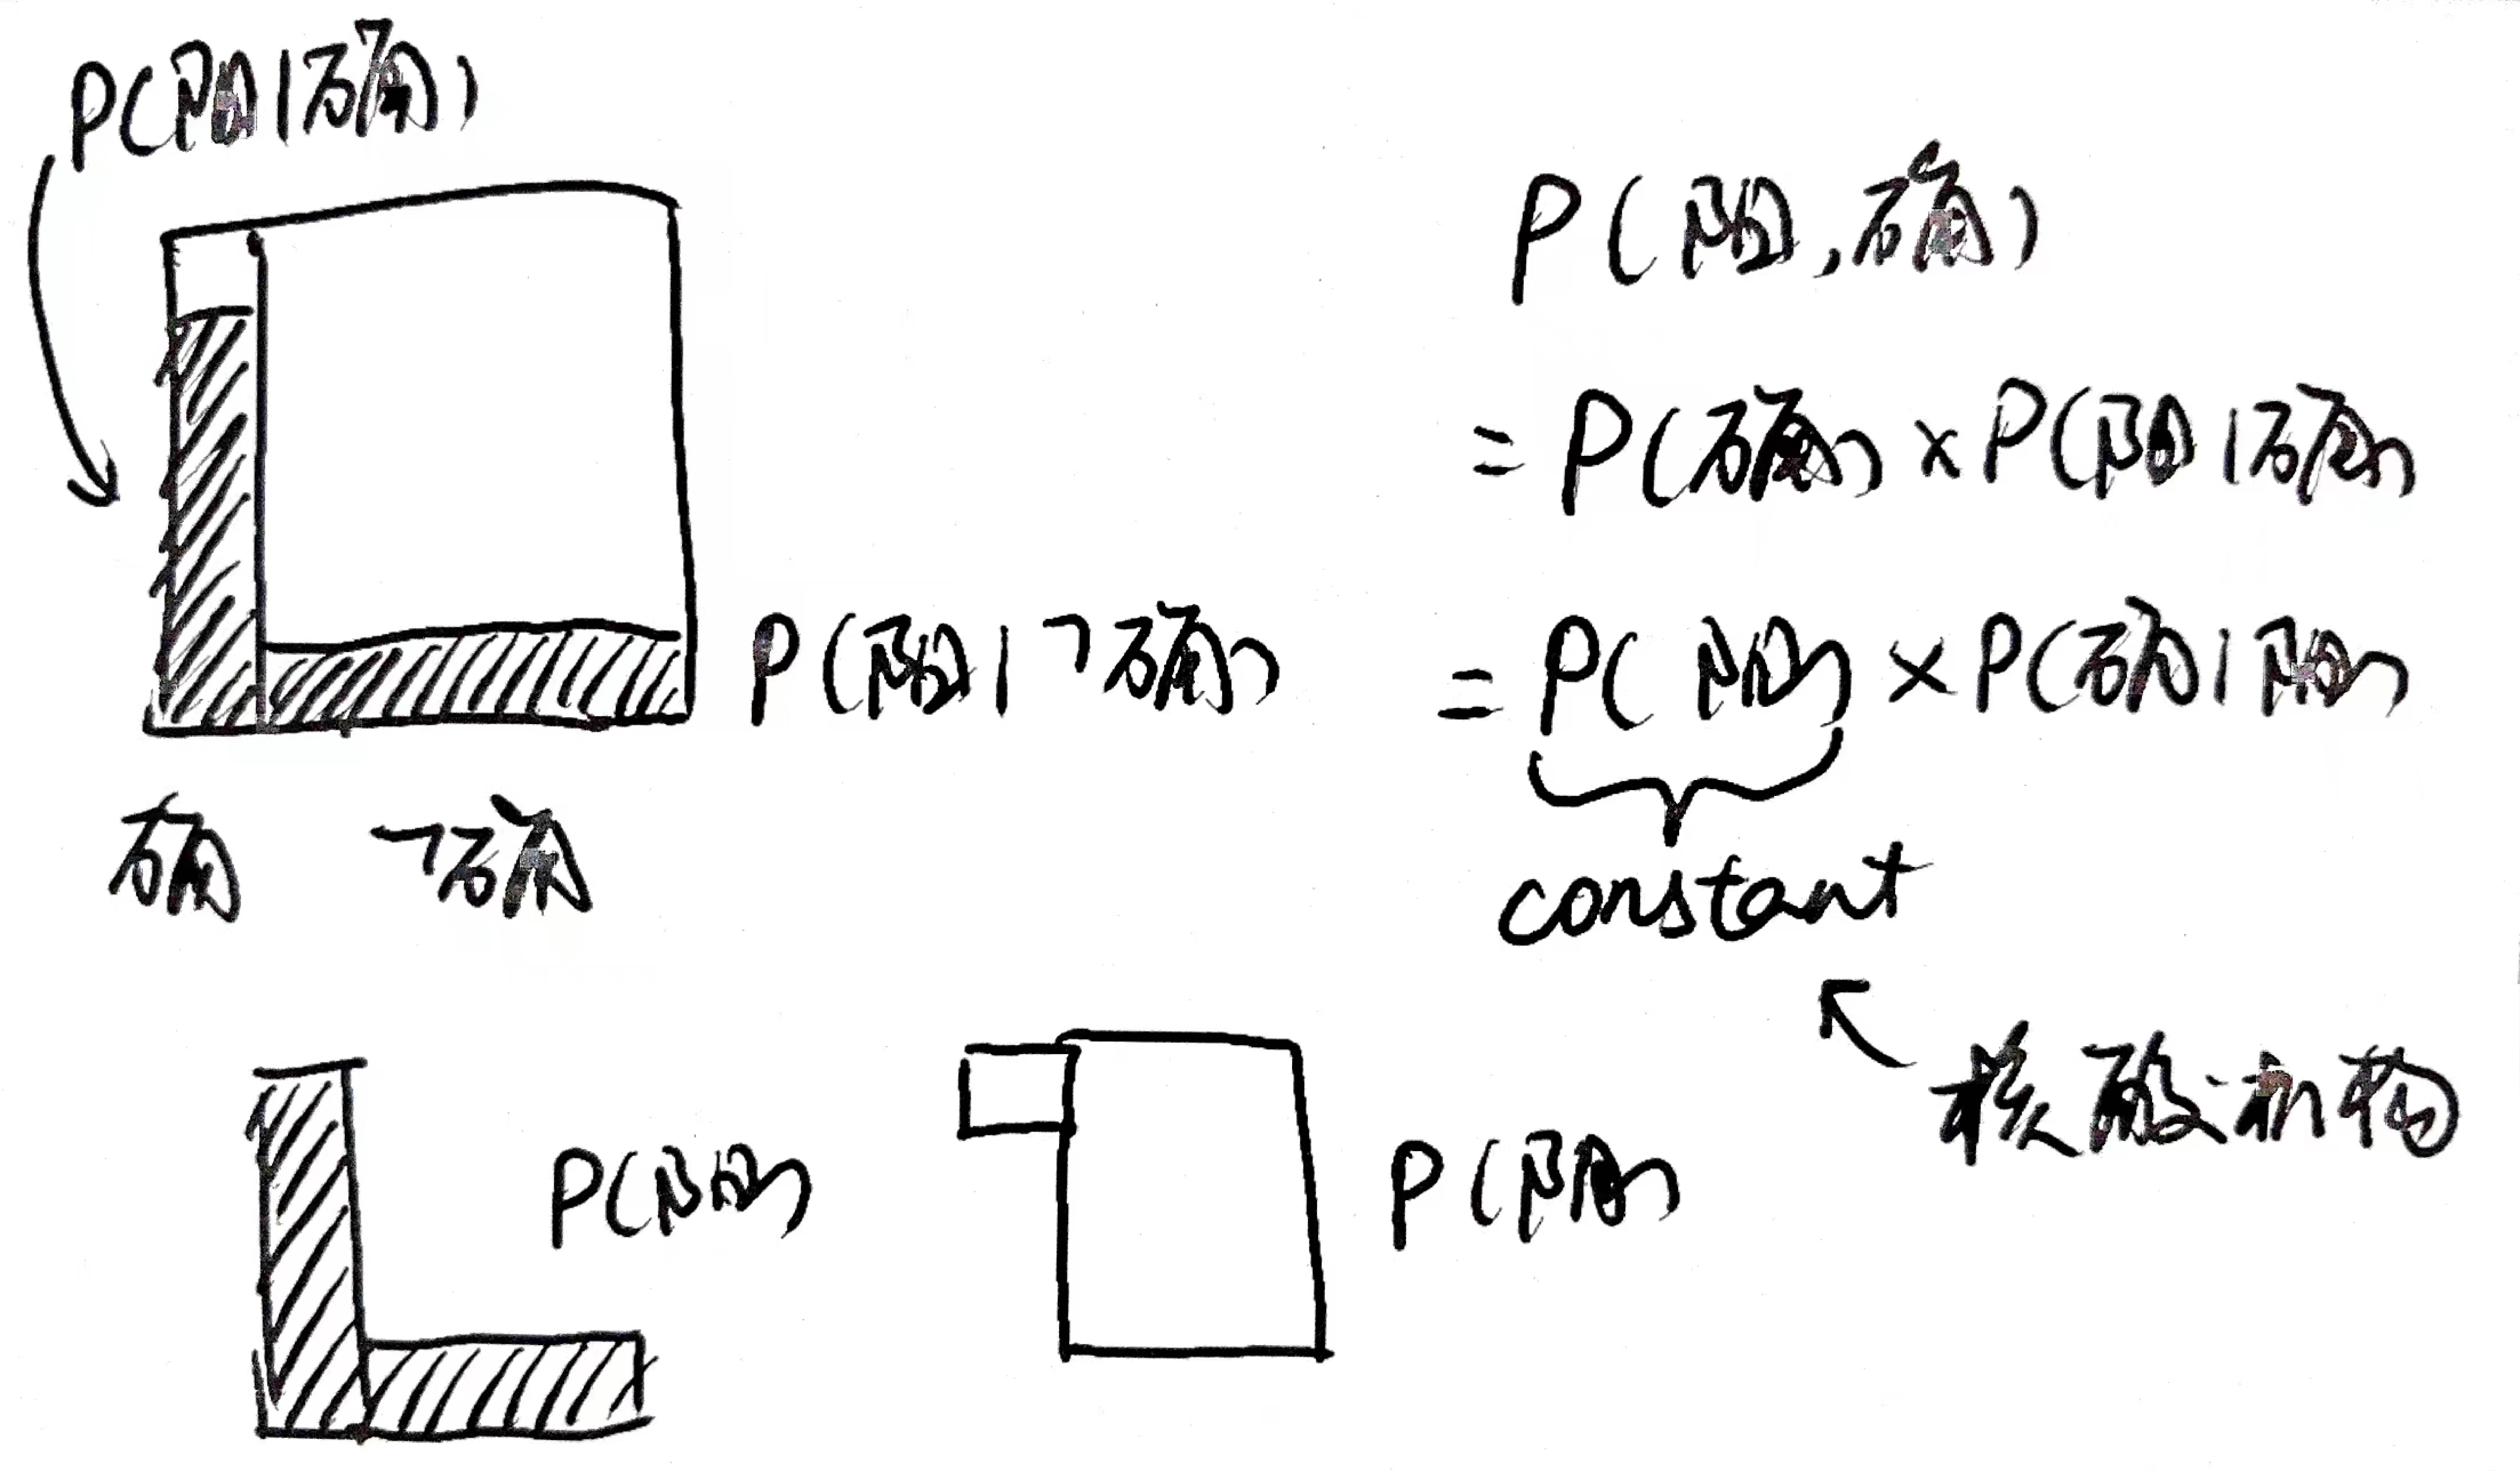
\includegraphics[width=0.8\textwidth]{fig7.jpg}
\end{center}

\begin{Answer}
	\begin{equation}
		\begin{aligned}
			P(\text{确诊}|\text{阳性})
			 & = \frac{P(\text{阳性}|\text{确诊}) \times P(\text{确诊})}{P(\text{阳性})}    \\
			 & = \frac{0.99 \times 0.0001}{0.99 \times 0.0001 + 0.01 \times 0.9999} \\
			 & = 0.0098
		\end{aligned}
	\end{equation}
\end{Answer}

\begin{Exercise}
	小贝\textbf{重做}核酸检测。已知小贝的确诊率为 0.0098,确诊人群的阳性率为 0.99,其他人的阳性率为 0.01。假设小贝的检测结果\textbf{又}为阳性,求小贝确诊的概率。
\end{Exercise}


\begin{center}
	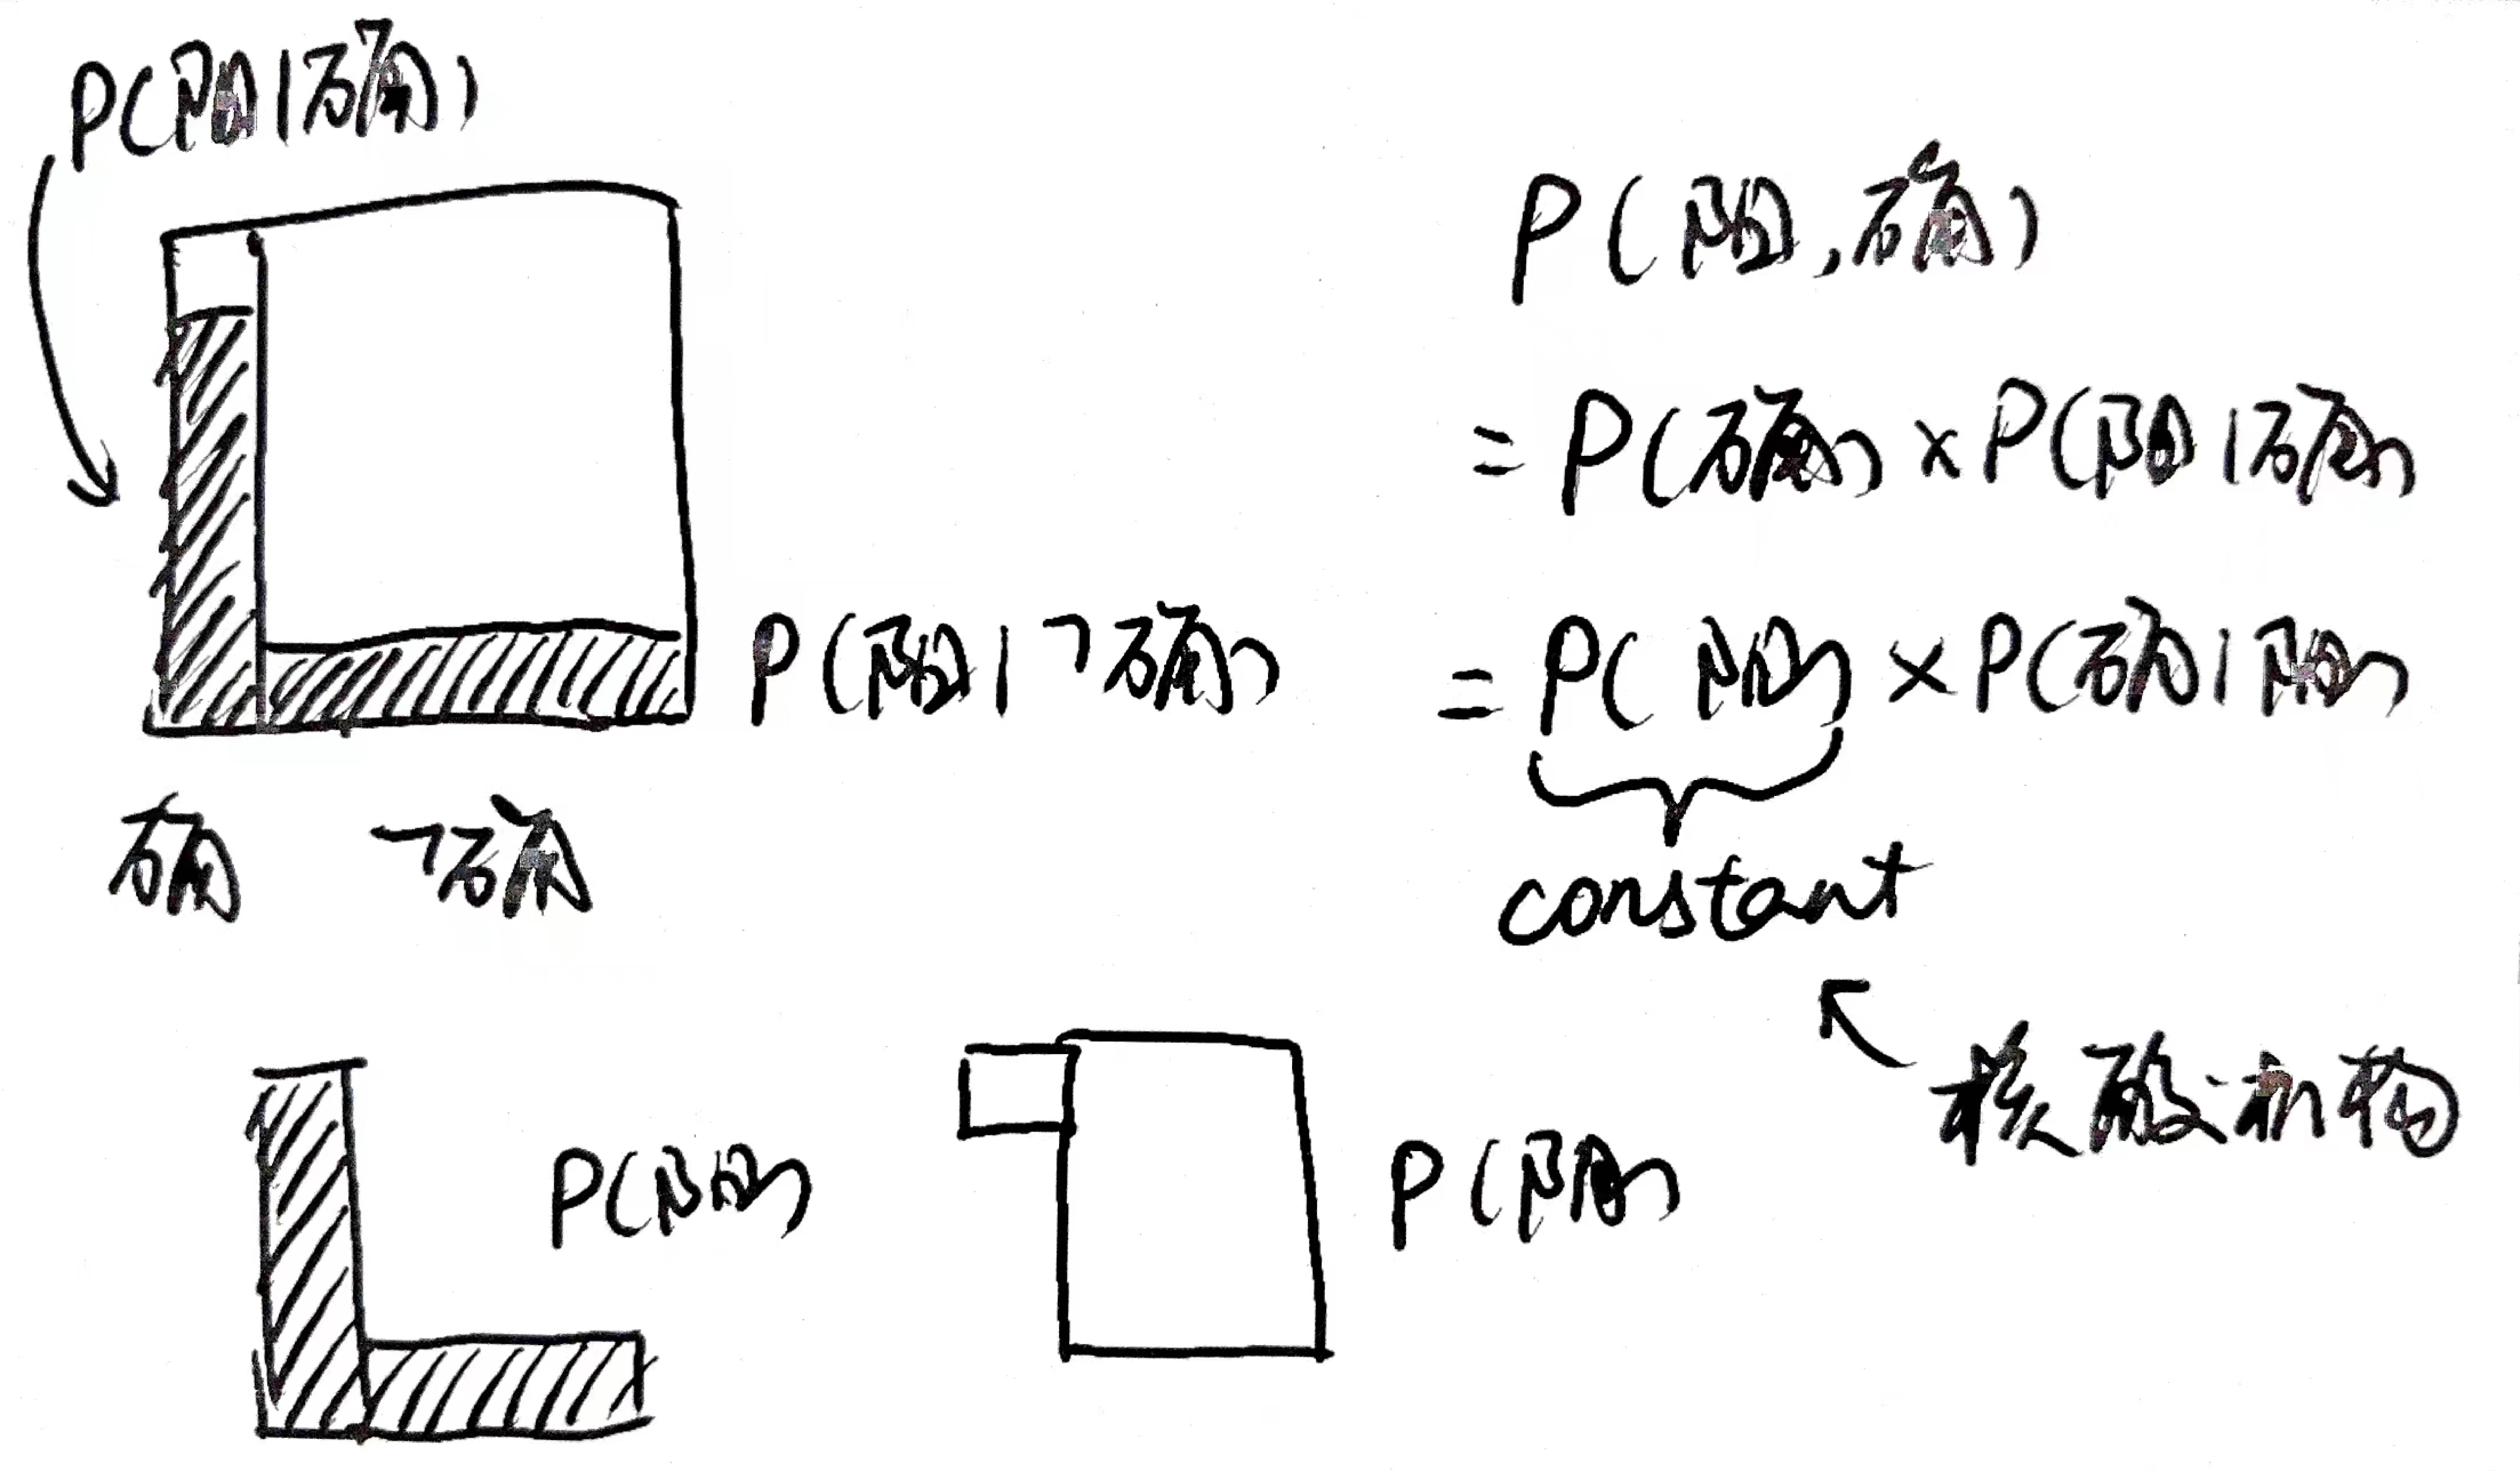
\includegraphics[width=0.8\textwidth]{fig7.jpg}
\end{center}

\begin{Answer}
	\begin{equation}
		\begin{aligned}
			P(\text{确诊}|\text{阳性})
			 & = \frac{P(\text{阳性}|\text{确诊}) \times P(\text{确诊})}{P(\text{阳性})}    \\
			 & = \frac{0.99 \times 0.0098}{0.99 \times 0.0098 + 0.01 \times 0.9902} \\
			 & = 0.4949
		\end{aligned}
	\end{equation}
\end{Answer}


\begin{Exercise}
	小贝\textbf{重做}核酸检测。已知小贝的确诊率为 0.4949,确诊人群的阳性率为 0.99,其他人的阳性率为 0.01。假设小贝的检测结果\textbf{又}为阳性,求小贝确诊的概率。
\end{Exercise}

\begin{center}
	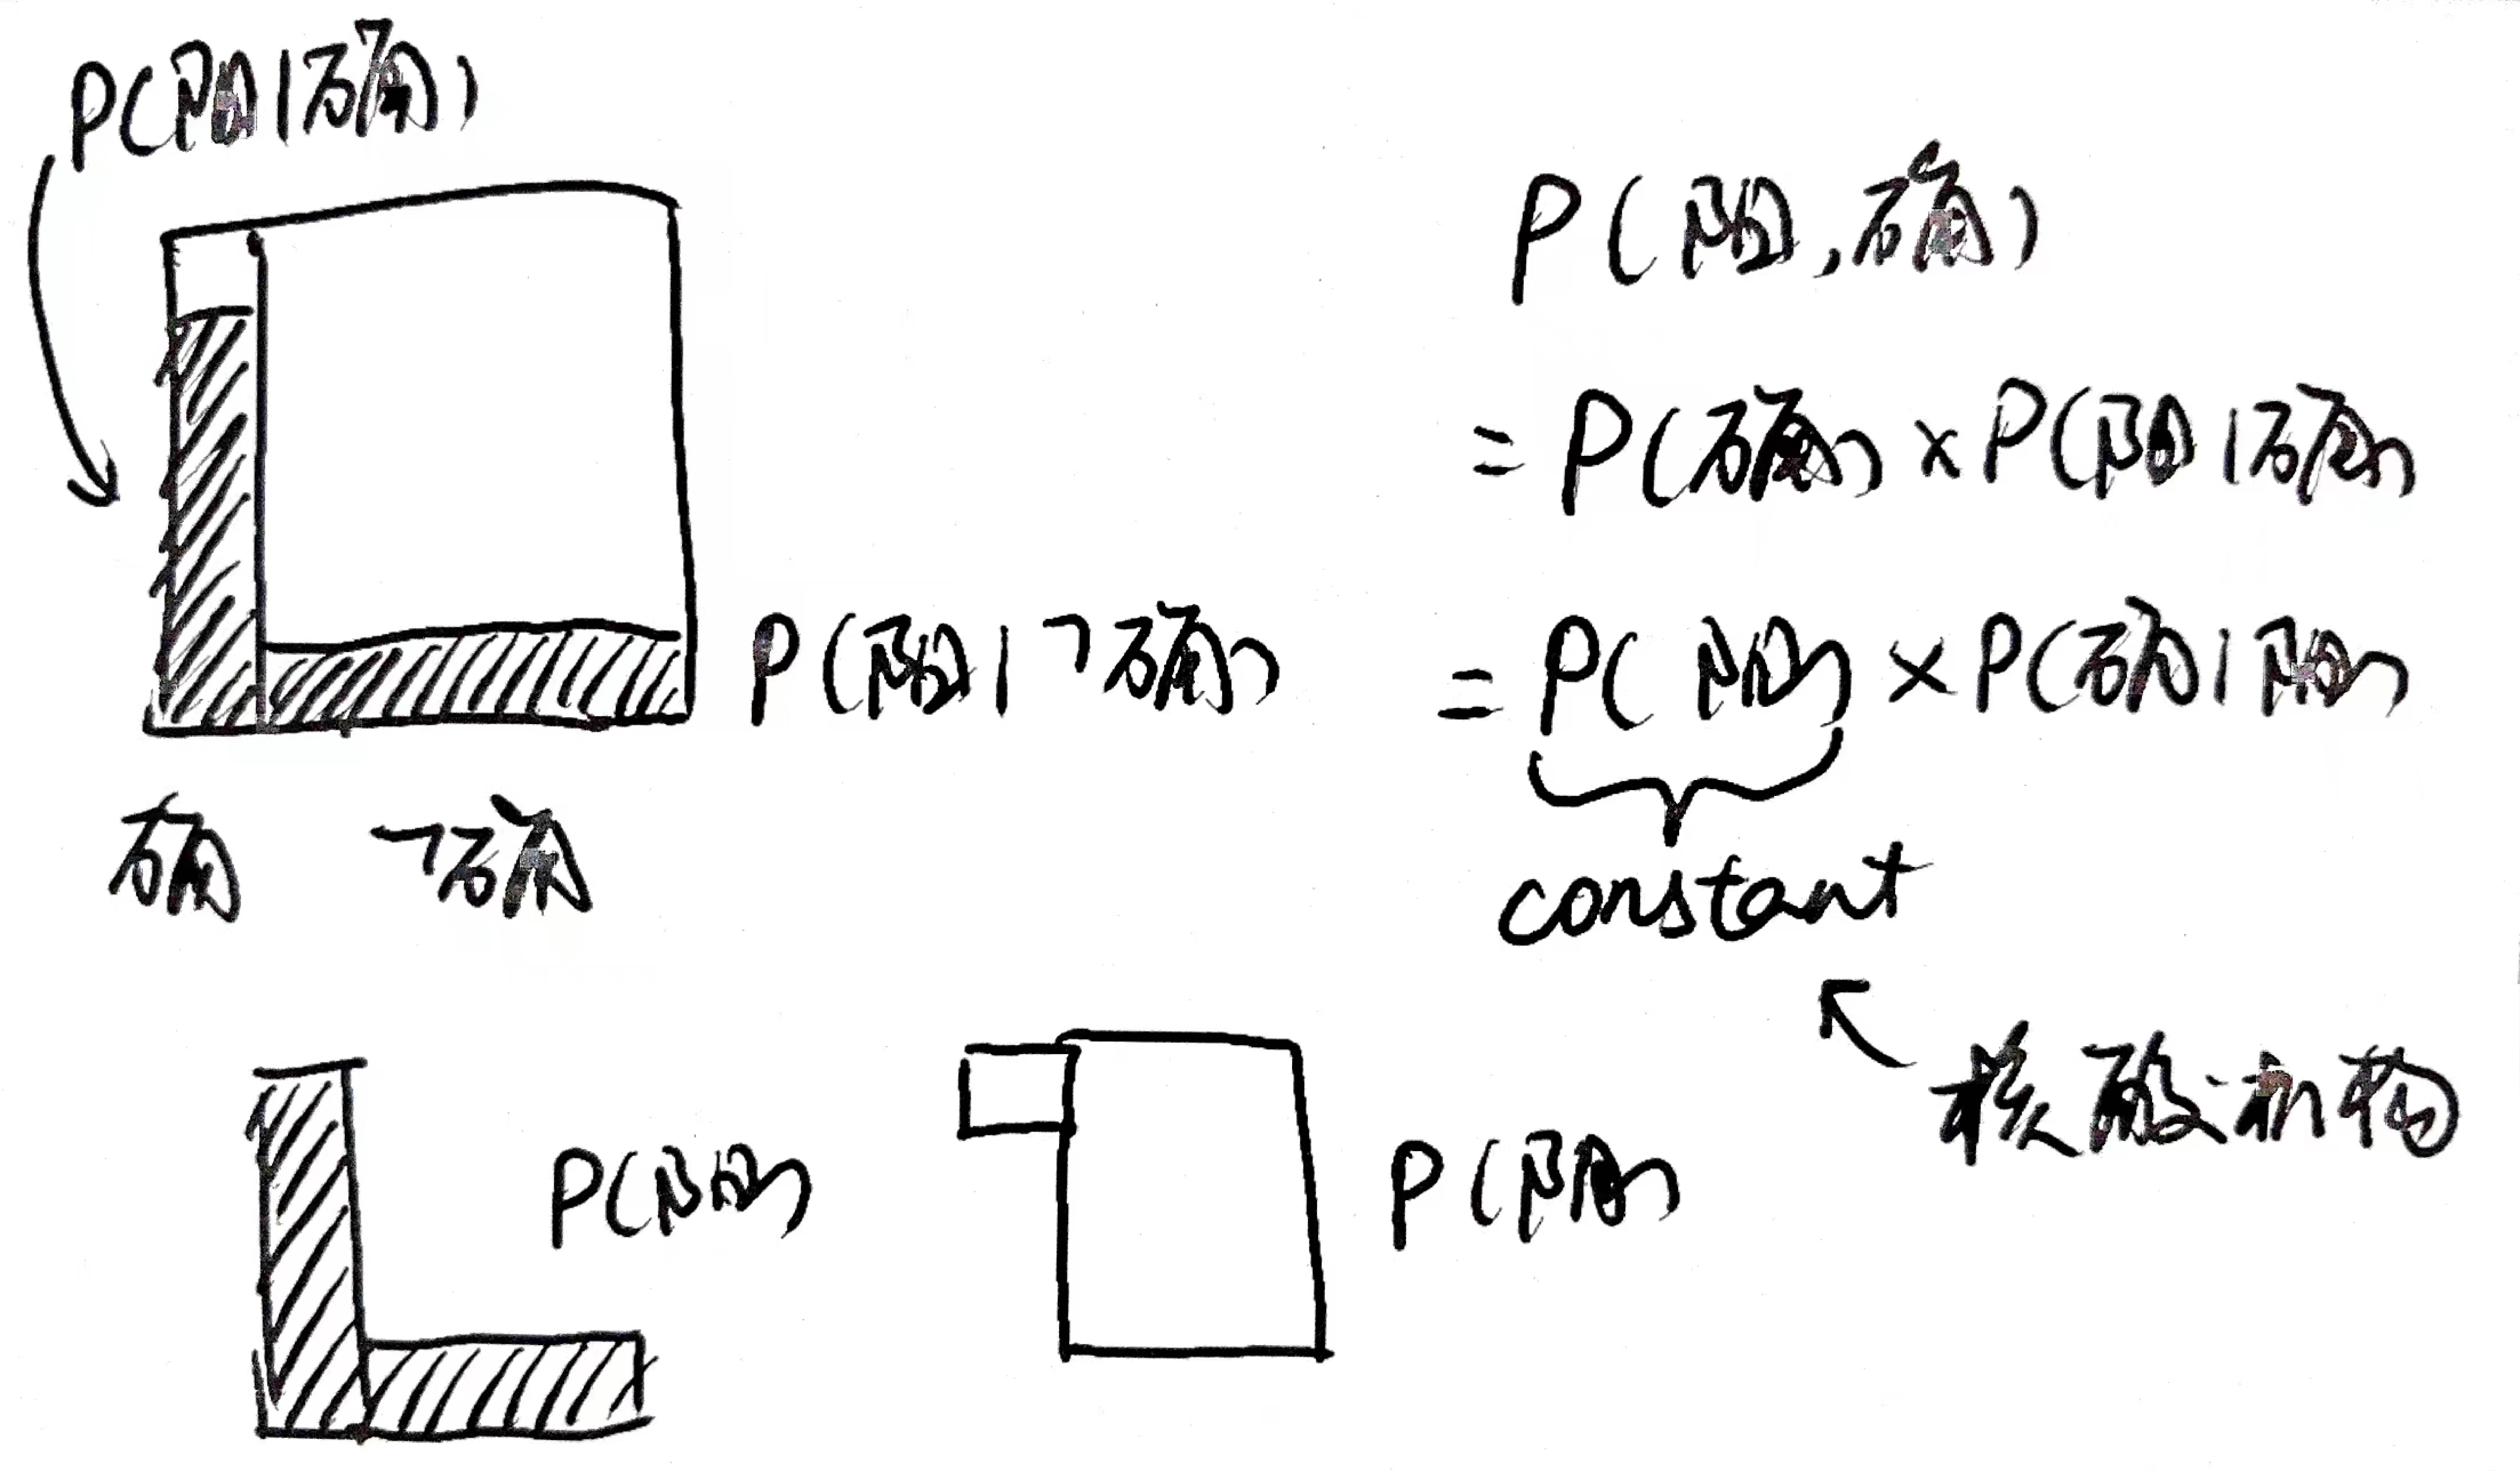
\includegraphics[width=0.8\textwidth]{fig7.jpg}
\end{center}

\begin{Answer}
	\begin{equation}
		\begin{aligned}
			P(\text{确诊}|\text{阳性})
			 & = \frac{P(\text{阳性}|\text{确诊}) \times P(\text{确诊})}{P(\text{阳性})}    \\
			 & = \frac{0.99 \times 0.4949}{0.99 \times 0.4949 + 0.01 \times 0.5051} \\
			 & = 0.99
		\end{aligned}
	\end{equation}
\end{Answer}

\subsection{案例二:大众点评}

在刚才的例子里,$P(\text{确诊})$ 一直在变化,这就是贝叶斯的思想。我们可以不断地更新我们的先验概率 $P(\text{确诊})$,从而得到更准确的后验概率。

举一个生活中的例子,假设我们在大众点评上看到了一个餐厅的评价,评分为 4.5 分。我们可以看看推荐菜,看看照片和价格,然后给出我们的心里的评分。

当我们真的去吃了以后,我们可以更新我们的评分。这就是贝叶斯的思想。

\begin{equation}
	\text{餐后评价} \propto \text{先验评价} \times \text{用餐体验}
\end{equation}

当然,如果我们后面又去吃了,我们可以再次更新我们的评分。

\begin{equation}
	\text{本次餐后评价} \propto \text{上次餐后评价} \times \text{用餐体验}
\end{equation}

\subsection{案例三:店铺好评}

\begin{Exercise}
	小贝逛淘宝看到一家新的店铺。这家店铺有 5 条好评,0 条差评,那么这家店铺的好评率应该是多少?
\end{Exercise}

\begin{Answer}
	这里我们没有任何先验信息,所以我们可以假设先验概率为 50\%。具体来说,我们假设一个Beta分布,$\text{Beta}(1, 1)$,即:

	\begin{center}
		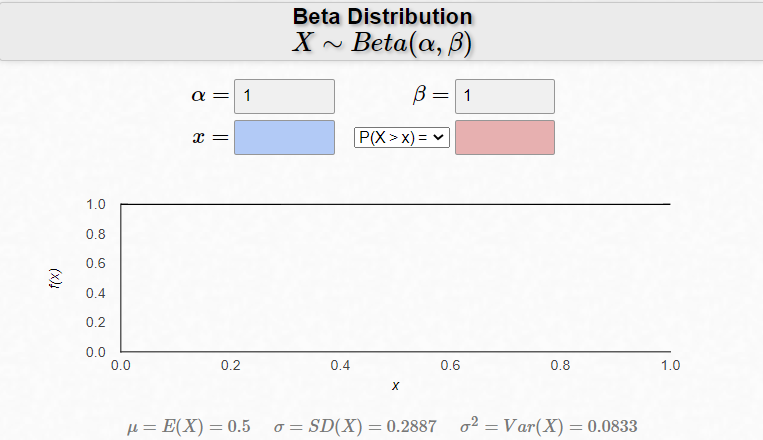
\includegraphics[width=0.8\textwidth]{fig11.png}
	\end{center}

	同时,数据告诉我们,这家店铺有 5 条好评,0 条差评,所以我们可以得到一个Beta分布,$\text{Beta}(5+1, 0+1)$,即:

	\begin{center}
		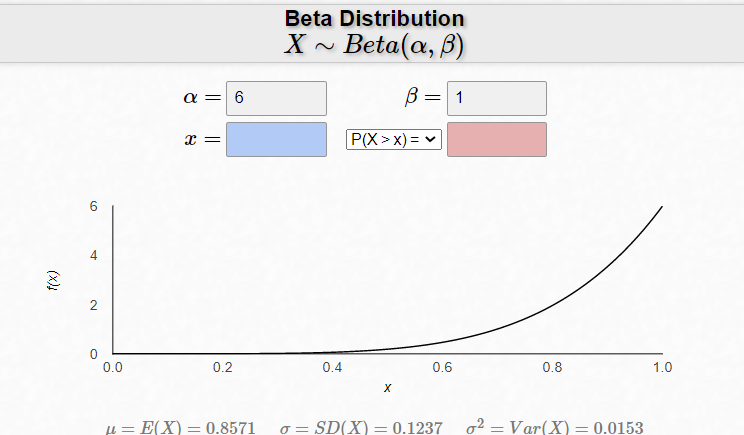
\includegraphics[width=0.8\textwidth]{fig12.png}
	\end{center}

	注:这两张图来自\href{https://homepage.divms.uiowa.edu/~mbognar/applets/beta.html}{Bognar (2021) 的网站}。

\end{Answer}

\begin{Exercise}
	小贝逛淘宝看到一家新的店铺。这家店铺有 90 条好评,10 条差评,那么这家店铺的好评率应该是多少?
\end{Exercise}

\begin{Answer}
	数据告诉我们,这家店铺有 90 条好评,10 条差评,所以我们可以得到一个Beta分布,$\text{Beta}(90+1, 10+1)$,即:

	\begin{center}
		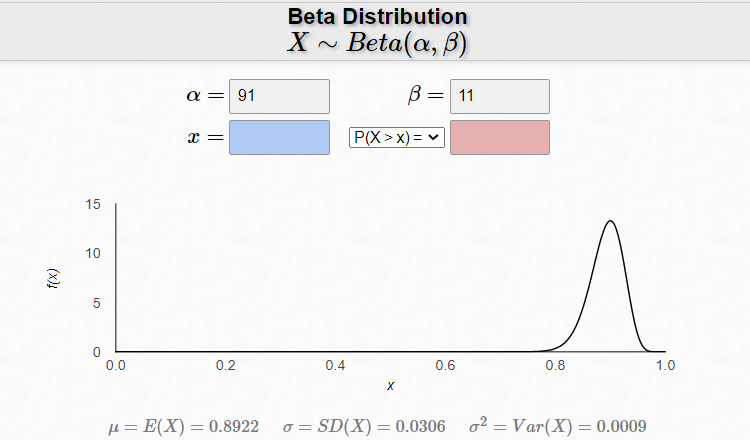
\includegraphics[width=0.8\textwidth]{fig13.png}
	\end{center}

\end{Answer}

\begin{Exercise}
	过了几天,小贝发现刚刚的店铺新增了5条好评。此时,这家店铺的好评率应该是多少?
\end{Exercise}

\begin{Answer}
	此时我们有个先验分布 $\text{Beta}(90+1, 10+1)$,然后我们有了新的数据,所以我们可以得到后验分布 $\text{Beta}(90+5+1, 10+1)$,即:

	\begin{center}
		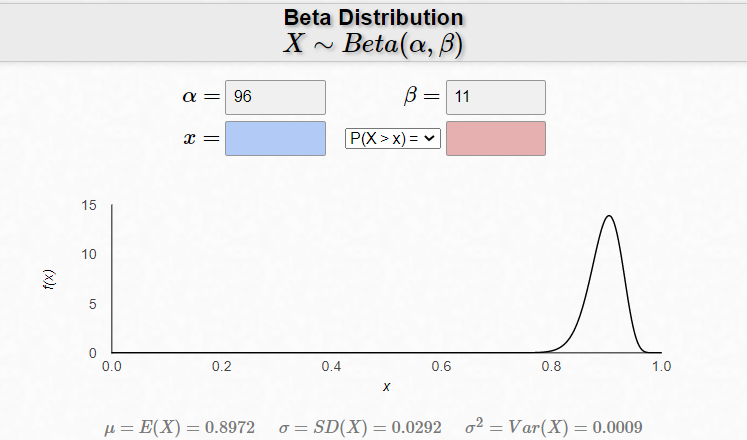
\includegraphics[width=0.8\textwidth]{fig14.png}
	\end{center}

\end{Answer}

显然,当我们的先验分布比较强时,我们的后验分布主要由先验分布决定;当我们的数据比较强时,我们的后验分布主要由数据决定。

\section{贝叶斯的优劣}

贝叶斯学派(Bayesian)和频率学派(Frequentist)是统计学中的两大学派。贝叶斯学派认为参数是随机的,而频率学派认为参数是固定的。

和频率学派相比,贝叶斯学派的优劣势如下:

\begin{itemize}
	\item 优点:
	      \begin{enumerate}
		      \item 不用提一个注定错误的假设($H_0: \beta = 0$),在原理上没有硬伤。
		      \item 可以证明一个东西没有影响(“不显著”)。
		      \item 可以纳入先验信息。
		      \item 更好地处理小样本问题。
		      \item 通过电脑模拟来估计系数,天然适配多层次模型等。
		      \item 可以拟合约束复杂的模型。
	      \end{enumerate}
	\item 缺点:
	      \begin{enumerate}
		      \item 需要大量数值计算,稍复杂的模型会跑很久。
		      \item 解释结果较为复杂,社会学界尚未普及。
		      \item 学习曲线陡峭,需要大量统计知识。
	      \end{enumerate}
\end{itemize}


\end{document}